
\chapter{Arquitetura de Software}
\label{sec-arquitetura}
\vspace{-1cm}

A Figura~\ref{figura-arquitetura} mostra a arquitetura do sistema \emph{\imprimirtitulo}.

\begin{figure}[h]
	\centering
	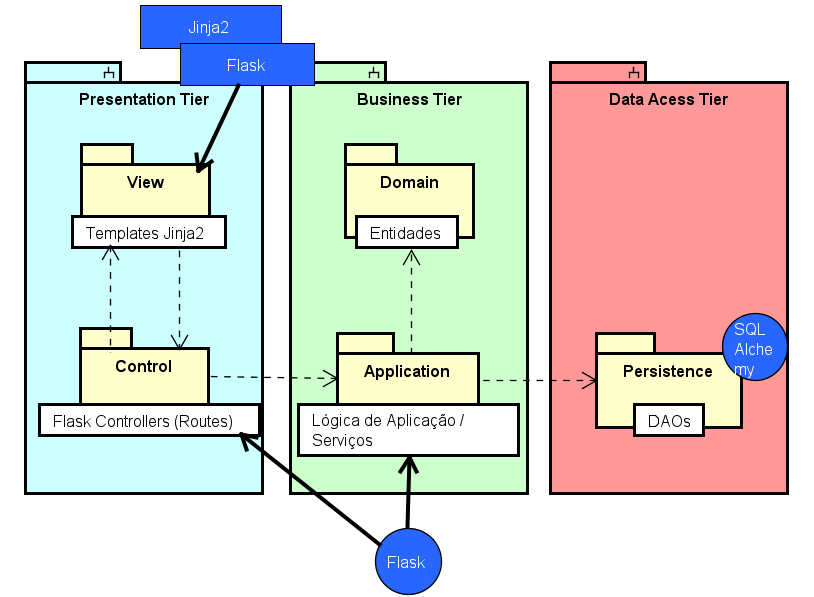
\includegraphics[width=0.8\textwidth]{figuras/figura_arquitetura.png}
	\caption{Arquitetura de Software.}
	\label{figura-arquitetura}
\end{figure}


A arquitetura de software representada no diagrama segue o padrão em três camadas, projetado para separar as responsabilidades da aplicação em módulos distintos: Apresentação, Negócio e Acesso a Dados. Essa estrutura resulta em um sistema mais organizado e de fácil manutenção.

A Camada de Apresentação é a interface com o usuário, responsável por processar requisições e renderizar a interface. Ela utiliza os Controllers do Flask para gerenciar as rotas e o motor de templates Jinja2 para exibir as páginas web. A Camada de Negócio, por sua vez, centraliza a lógica e as regras do sistema, sendo composta pelas Entidades de Domínio e pelos Serviços de Aplicação que orquestram as operações.

Por fim, a Camada de Acesso a Dados gerencia a persistência dos dados, abstraindo a comunicação com o banco de dados. Ela utiliza DAOs (Data Access Objects) e o framework SQLAlchemy como ORM (Mapeamento Objeto-Relacional). O framework Flask atua como o elemento central, gerenciando o fluxo entre a apresentação e o negócio, garantindo que as camadas permaneçam desacopladas e coesas.